% UATD sonar detection: RF-DETR project update.
% Tables in generated/ and figures in figures/ are produced by
%   python scripts/make_report_assets.py ...   (do not edit them by hand; re-run the script)
% Yellow "Write this in your own words" boxes mark the text the students must write.
% Compile with pdfLaTeX (Overleaf default) or Tectonic.
\documentclass[11pt,a4paper]{article}

\usepackage[T1]{fontenc}
\usepackage[utf8]{inputenc}
\usepackage{lmodern}
\usepackage[margin=2.3cm,headheight=14pt]{geometry}
\usepackage{graphicx}
\usepackage{booktabs}
\usepackage{longtable}
\usepackage{array}
\usepackage{amsmath}
\usepackage{xcolor}
\usepackage{float}
\usepackage{caption}
\usepackage{fancyhdr}
\usepackage{titlesec}
\usepackage{enumitem}
\usepackage[most]{tcolorbox}
\usepackage{tikz}
\usetikzlibrary{positioning,arrows.meta,shapes.misc}
\usepackage[hidelinks]{hyperref}

\definecolor{accent}{HTML}{1F6F8B}
\definecolor{muted}{HTML}{6B7785}
\captionsetup{font=small,labelfont=bf}
\setlist{nosep}

\pagestyle{fancy}
\fancyhf{}
\fancyhead[L]{\small\color{muted}UATD / RF-DETR \textbullet{} Project Update}
\fancyhead[R]{\small\color{muted}\thepage}
\fancyfoot[L]{\scriptsize\color{muted}Numbers generated from run \texttt{small\_rdefault\_s0} by the shared evaluator}
\renewcommand{\headrulewidth}{0.4pt}

\titleformat{\section}{\Large\bfseries\color{accent}}{\thesection}{0.8em}{}
\titleformat{\subsection}{\large\bfseries\color{accent}}{\thesubsection}{0.6em}{}

% Placeholder for text the students write themselves (CLAUDE.md rule 4).
\newtcolorbox{writehere}{enhanced,breakable,colback=yellow!8,colframe=orange!75!black,
  fonttitle=\bfseries\small,title={Write this in your own words},fontupper=\small}

\newcommand{\gentab}[1]{\input{generated/#1}}

\begin{document}

% ------------------------------------------------------------------ title page
\begin{titlepage}
\centering
\vspace*{1.5cm}
% \includegraphics[width=2.6cm]{figures/nsu_logo.png}\\[0.6cm]  % add the logo file to use it
{\Large\bfseries North South University}\\[2pt]
Department of Electrical \& Computer Engineering\\[1.4cm]
\rule{\linewidth}{0.4pt}\\[0.4cm]
{\Huge\bfseries Project Update}\\[0.3cm]
\rule{\linewidth}{0.4pt}\\[1.2cm]
{\LARGE\bfseries Underwater Sonar Object Detection using\\[4pt] RF-DETR}\\[1.2cm]
\begin{tabular}{rl}
\textbf{Course} & CSE 499A, Section 12\\
\textbf{Supervisor} & Dr.\ Riasat Khan
\end{tabular}\\[1.4cm]
\begin{tabular}{lll}
\toprule
\textbf{Student Name} & \textbf{Student ID} & \textbf{Email}\\
\midrule
Walidur Rahman & 231 1712 642 & walidur.rahman01@northsouth.edu\\
Mridha Fahad Hossain & 231 2199 042 & mridha.hossain@northsouth.edu\\
Nafsin Nasama Salmee & 231 1776 642 & nafsin.salmee@northsouth.edu\\
Md.\ Azmine Amin Mormo & 231 2318 042 & azmine.mormo@northsouth.edu\\
\bottomrule
\end{tabular}\\[1.4cm]
\textbf{Submission Date:} \today
\end{titlepage}

\tableofcontents
\newpage

% ------------------------------------------------------------------ 1 overview
\section{Overview}
\subsection{Executive summary}
\begin{writehere}
Points to cover:
\begin{itemize}
  \item Task: 10-class object detection on UATD forward-looking sonar images.
  \item Main pipeline: RF-DETR (Robinson et al., ICLR 2026), Small model, DINOv2 backbone, fine-tuned from COCO weights.
  \item Same fixed split as the YOLO26n baseline; all numbers from one shared COCO evaluator; test sets never used for training or selection.
  \item Headline: test1 mAP50 0.815 (YOLO26n 0.777), test2 0.825 (YOLO26n 0.804); mAP50:95 0.368 / 0.363 (YOLO26n 0.329 / 0.337).
  \item Main remaining problems: cage classes, localisation at strict IoU (mAP75 0.26 / 0.25).
\end{itemize}
\end{writehere}

\begin{table}[H]\centering
\caption{Headline detection performance of RF-DETR-S (mAP at IoU 0.5).}
\gentab{tab_headline}
\end{table}

\begin{table}[H]\centering
\caption{RF-DETR-S versus the YOLO26n reference on the same split.
$^\dagger$YOLO26n values are copied from the original notebook (Ultralytics validator, imgsz 640); RF-DETR values come from our shared evaluator (pycocotools + Ultralytics-definition P/R/F1).}
\label{tab:vsyolo}
\gentab{tab_vs_yolo}
\end{table}

\subsection{Objectives}
\begin{writehere}
Points to cover: reproduce the fixed split exactly; train a peer-reviewed transformer detector (RF-DETR) as the main pipeline; evaluate every model with one shared evaluator; identify weak classes and the size/localisation gap; prepare for baselines (YOLOv12, FBRT-YOLO, DEIM-D-FINE, Dome-DETR) and a tiny-object method.
\end{writehere}

% ------------------------------------------------------------------ 2 dataset
\section{Dataset}
\subsection{Fixed split and cleaning}
\begin{writehere}
Points to cover: UATD (figshare 21331143), 7{,}600 training + 800 Test~1 + 800 Test~2 images, VOC XML; validation = first 760 of the seed-42 shuffle of the training stems (same as the YOLO26n notebook); cleaning swaps 8 reversed boxes, clips 2, drops 11 images with zero-area boxes; split verified by automated tests against the expected counts.
\end{writehere}

\begin{table}[H]\centering
\caption{Images and objects per split after cleaning.}
\gentab{tab_dataset}
\end{table}

\begin{table}[H]\centering
\caption{Objects per class and split.}
\gentab{tab_class_counts}
\end{table}

\subsection{Image and box statistics}
\begin{figure}[H]\centering
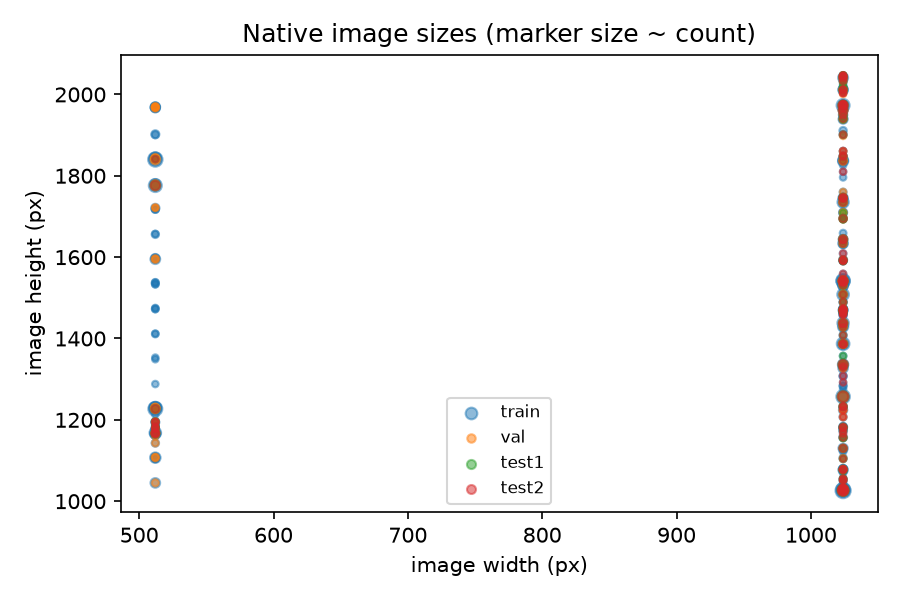
\includegraphics[width=0.49\linewidth]{figures/image_sizes.png}\hfill
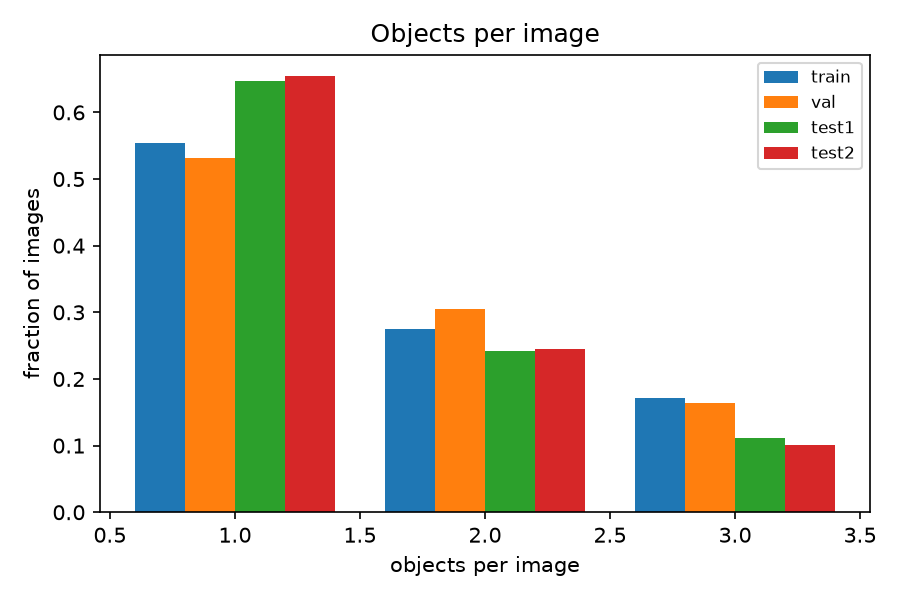
\includegraphics[width=0.49\linewidth]{figures/objects_per_image.png}
\caption{Native image sizes (224 distinct sizes; width 512 or 1024, height 1024--2047) and objects per image.}
\end{figure}

\begin{figure}[H]\centering
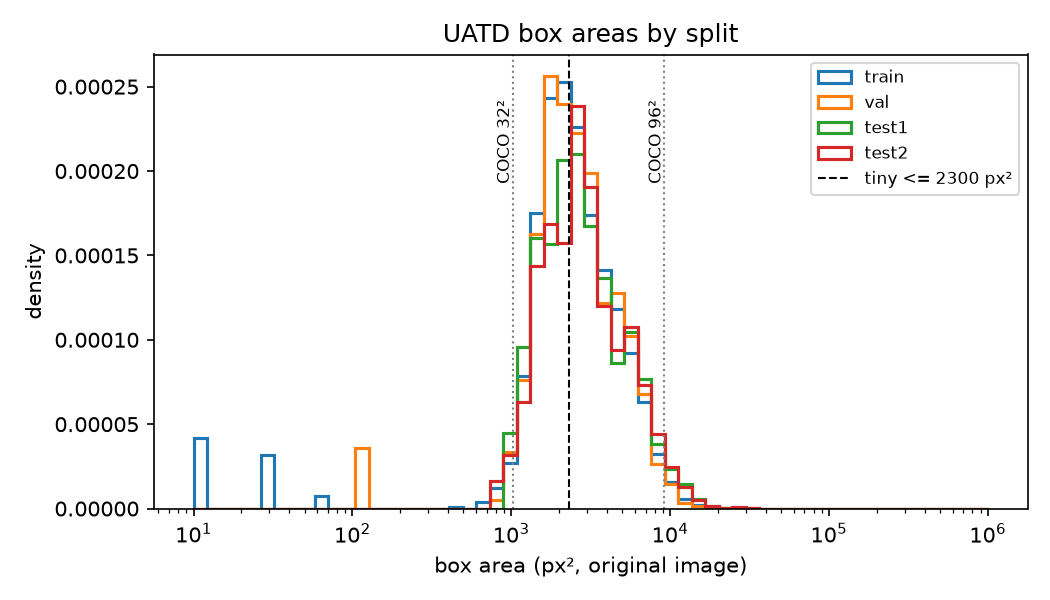
\includegraphics[width=0.49\linewidth]{figures/box_area_by_split.png}\hfill
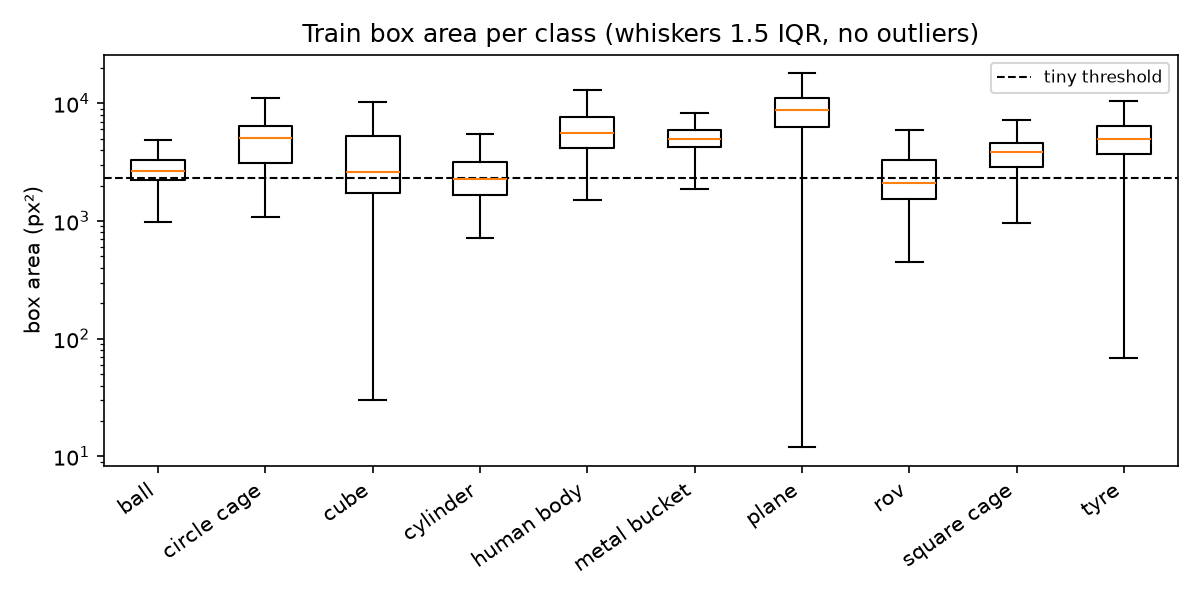
\includegraphics[width=0.49\linewidth]{figures/box_area_per_class_train.png}
\caption{Box area per split and per class (train). The dashed line marks the tiny threshold (2300\,px$^2$, the 25th percentile of train box areas).}
\end{figure}

\begin{writehere}
Points to cover: median box 58$\times$62\,px; 94\% of train boxes fall in COCO ``medium'', so COCO's absolute bins say little; tiny defined as area $\leq$ 2300\,px$^2$ ($\approx$48$\times$48\,px), frozen in \texttt{configs/eval.yaml} before any model was evaluated; tiny fraction train 25\%, val 25\%, test1 20\%, test2 18\%; at 512$\times$512 input the median box shrinks to about 38$\times$21\,px.
\end{writehere}

% ------------------------------------------------------------------ 3 methodology
\section{Methodology}
\subsection{Pipeline}
\begin{figure}[H]\centering
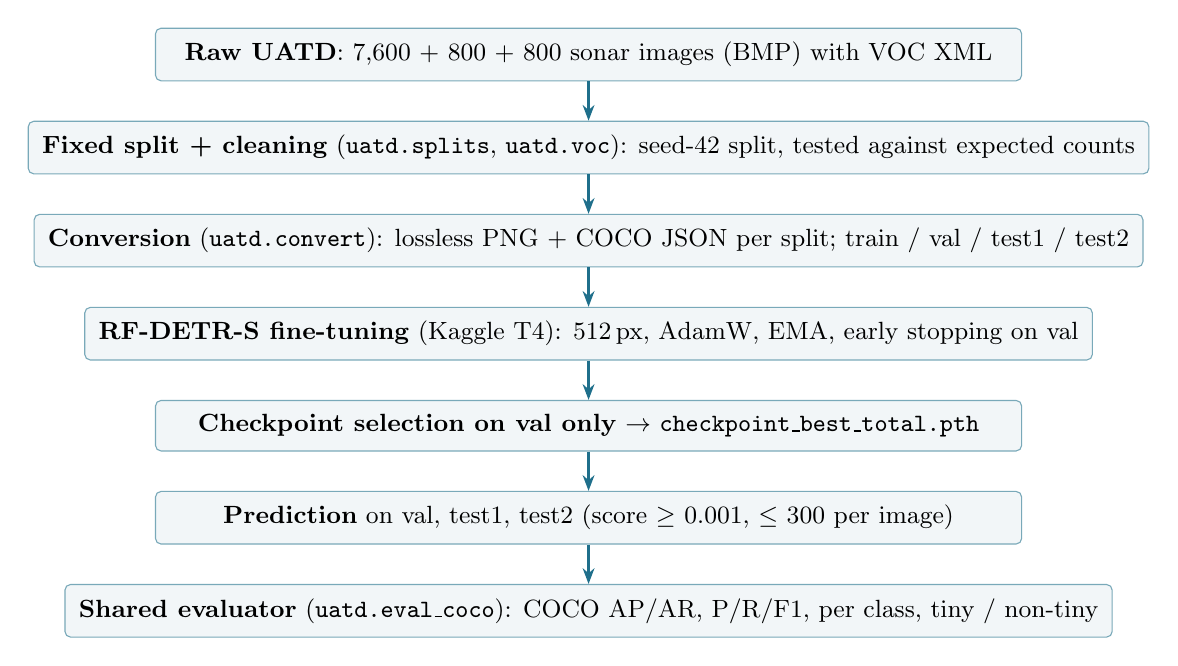
\begin{tikzpicture}[
  node distance=5mm,
  box/.style={draw=accent!60,fill=accent!6,rounded corners=2pt,minimum width=11cm,align=center,font=\small,inner sep=5pt},
  arr/.style={-{Stealth[length=2mm]},accent,thick}]
\node[box] (a) {\textbf{Raw UATD}: 7{,}600 + 800 + 800 sonar images (BMP) with VOC XML};
\node[box,below=of a] (b) {\textbf{Fixed split + cleaning} (\texttt{uatd.splits}, \texttt{uatd.voc}): seed-42 split, tested against expected counts};
\node[box,below=of b] (c) {\textbf{Conversion} (\texttt{uatd.convert}): lossless PNG + COCO JSON per split; train / val / test1 / test2};
\node[box,below=of c] (d) {\textbf{RF-DETR-S fine-tuning} (Kaggle T4): 512\,px, AdamW, EMA, early stopping on val};
\node[box,below=of d] (e) {\textbf{Checkpoint selection on val only} $\rightarrow$ \texttt{checkpoint\_best\_total.pth}};
\node[box,below=of e] (f) {\textbf{Prediction} on val, test1, test2 (score $\geq$ 0.001, $\leq$ 300 per image)};
\node[box,below=of f] (g) {\textbf{Shared evaluator} (\texttt{uatd.eval\_coco}): COCO AP/AR, P/R/F1, per class, tiny / non-tiny};
\foreach \u/\v in {a/b,b/c,c/d,d/e,e/f,f/g} \draw[arr] (\u) -- (\v);
\end{tikzpicture}
\caption{End-to-end pipeline. Test1 and test2 enter only at the prediction step.}
\end{figure}

\subsection{RF-DETR}
\begin{writehere}
Points to cover (cite the ICLR 2026 paper): DETR-style detector; DINOv2 ViT backbone with windowed attention; multi-scale projector; deformable-attention decoder (3 layers, 300 queries); two-stage query initialisation; set-based (Hungarian) matching, so no NMS; losses = classification (IA-BCE) + L1 box + GIoU, with auxiliary losses on every decoder layer; Group-DETR training (13 query groups); model sizes from a weight-sharing architecture search. Why chosen: peer-reviewed A* venue, different family from RT-DETR (classmate), designed to transfer to new domains.
\end{writehere}

\begin{table}[H]\centering
\caption{Model and training configuration (from \texttt{training\_config.json} and \texttt{run\_config.json}).}
\gentab{tab_train_config}
\end{table}

\subsection{Evaluation protocol}
\begin{table}[H]\centering
\caption{Metrics reported by the shared evaluator.}
\begin{tabular}{p{3.4cm}p{10.6cm}}
\toprule
Metric & Definition used\\
\midrule
mAP50:95, mAP50, mAP75 & pycocotools, 101-point interpolation, max 100 detections per image\\
AP\textsubscript{S/M/L}, AR & pycocotools with COCO's absolute area bins ($32^2$, $96^2$)\\
P, R, F1 & Ultralytics definition (as used for YOLO26n): IoU 0.5, greedy matching by confidence, class-mean P and R at the confidence that maximises the smoothed mean F1\\
Per class & AP50, AP50:95, P, R, F1, number of GT boxes\\
Tiny / non-tiny AP & pycocotools with area bins $[0, 2300]$ and $(2300, \infty)$\,px$^2$, frozen before evaluation\\
Efficiency & params, GFLOPs, T4 batch-1 latency (FP16 / FP32): pending, see Section~\ref{sec:eff}\\
\bottomrule
\end{tabular}
\end{table}

% ------------------------------------------------------------------ 4 training
\section{Training}
\begin{table}[H]\centering
\caption{Execution environment and run summary.}
\gentab{tab_environment}
\end{table}

\begin{figure}[H]\centering
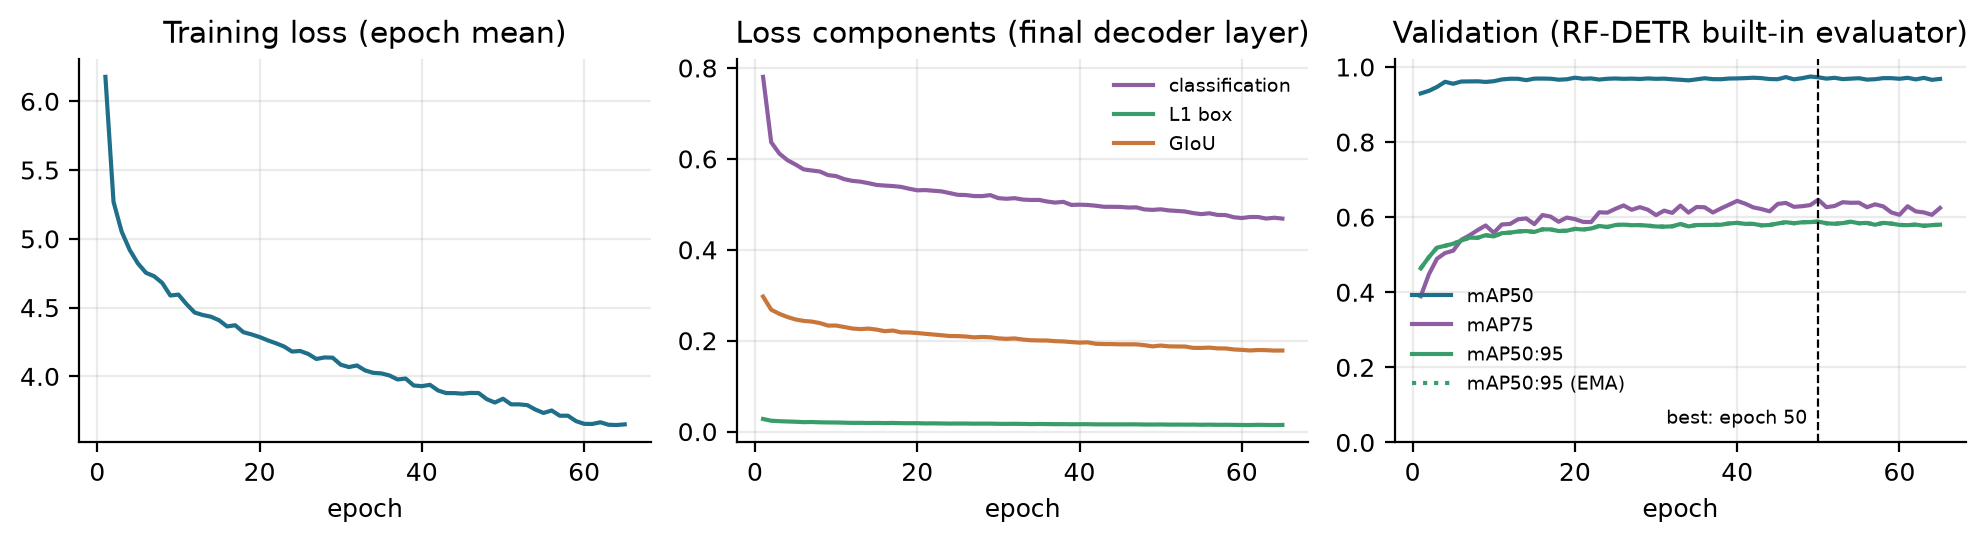
\includegraphics[width=\linewidth]{figures/fig_training_curves.png}
\caption{Training losses and validation metrics per epoch (RF-DETR's built-in evaluator, used only for monitoring and checkpoint selection). The dashed line marks the selected epoch.}
\end{figure}

\begin{writehere}
Points to cover: 65 epochs in 7.4\,h, one session; early stopping (patience 15) after no val improvement since epoch 50; losses still falling at the end while val mAP50:95 flat at $\approx$0.58--0.59; val mAP50 above 0.93 from the first epoch (pretrained weights); full per-epoch log in Appendix~\ref{app:epochs}.
\end{writehere}

% ------------------------------------------------------------------ 5 evaluation
\section{Evaluation}
\subsection{Overall results}
\begin{table}[H]\centering
\caption{RF-DETR-S overall performance (shared evaluator).}
\gentab{tab_overall}
\end{table}

\begin{figure}[H]\centering
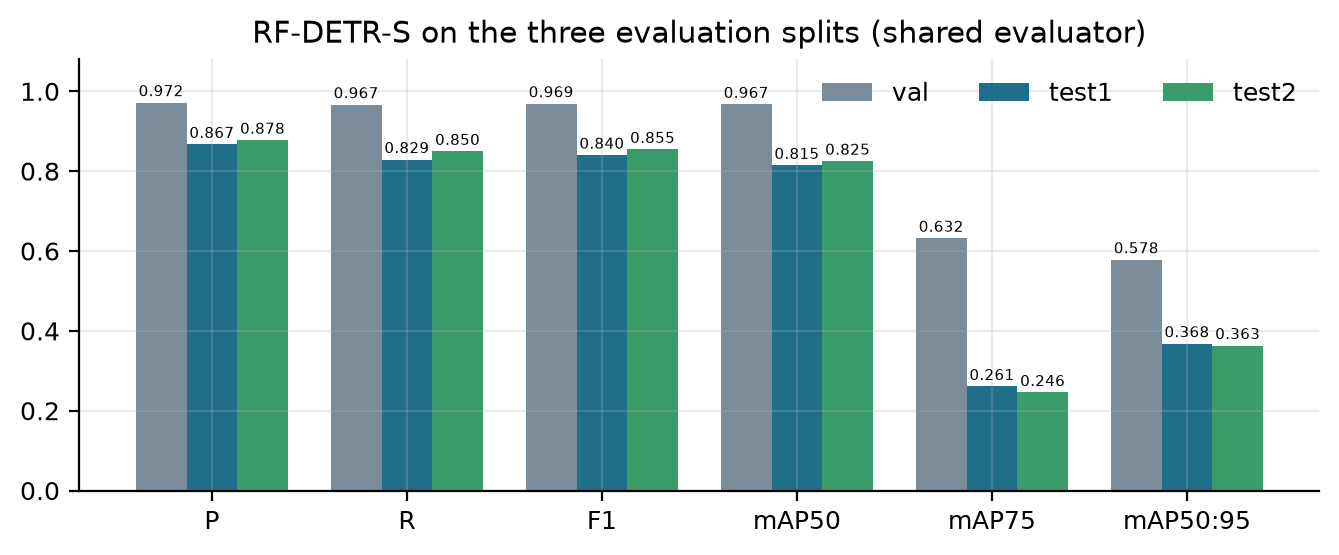
\includegraphics[width=0.9\linewidth]{figures/fig_split_comparison.png}
\caption{Validation versus held-out performance.}
\end{figure}

\begin{writehere}
Points to cover: val $\rightarrow$ test drop (mAP50 0.967 $\rightarrow$ 0.815 / 0.825; mAP50:95 0.578 $\rightarrow$ 0.368 / 0.363); val images come from the same collection as train, test sets were collected separately, so val overestimates; relative to YOLO26n (Table~\ref{tab:vsyolo}) RF-DETR is higher on every test metric, largest gains in mAP75 (+0.053 / +0.042) and mAP50 (+0.038 / +0.021); one seed only so far.
\end{writehere}

\subsection{Per-class results}
\begin{table}[H]\centering
\caption{Per-class results on validation.}
\gentab{tab_per_class_val}
\end{table}

\begin{table}[H]\centering
\caption{Per-class results on Test 1.}
\gentab{tab_per_class_test1}
\end{table}

\begin{table}[H]\centering
\caption{Per-class results on Test 2. Metal bucket has only 5 GT boxes.}
\gentab{tab_per_class_test2}
\end{table}

\begin{table}[H]\centering\small
\caption{Per-class AP on the test sets: YOLO26n reference (notebook, Ultralytics validator) versus RF-DETR-S (shared evaluator).}
\setlength{\tabcolsep}{4pt}
\gentab{tab_per_class_vs_yolo}
\end{table}

\begin{figure}[H]\centering
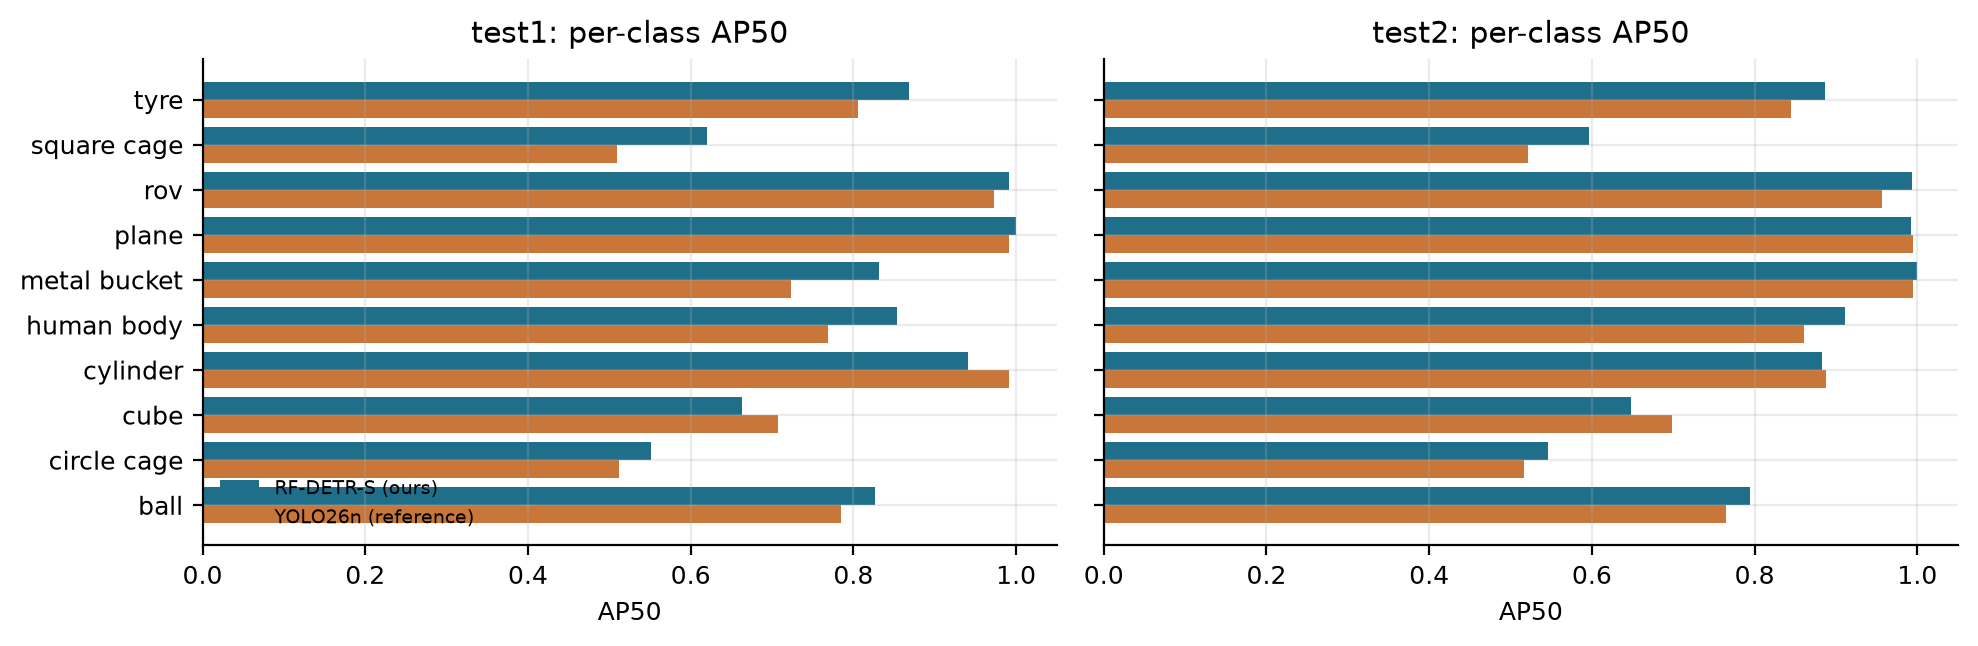
\includegraphics[width=\linewidth]{figures/fig_per_class_vs_yolo.png}
\caption{Per-class AP50 on Test 1 and Test 2.}
\end{figure}

\begin{writehere}
Points to cover: weakest classes on both tests are circle cage (AP50 0.551 / 0.546), square cage (0.620 / 0.596) and cube (0.663 / 0.648); square cage improves most over YOLO26n (+0.11 / +0.07), cube is slightly lower than YOLO26n (0.663 vs 0.708, 0.648 vs 0.699); plane, rov, cylinder near-perfect; metal bucket has only 6 / 5 test boxes, so its AP is unreliable.
\end{writehere}

\subsection{Precision--recall curves}
\begin{figure}[H]\centering
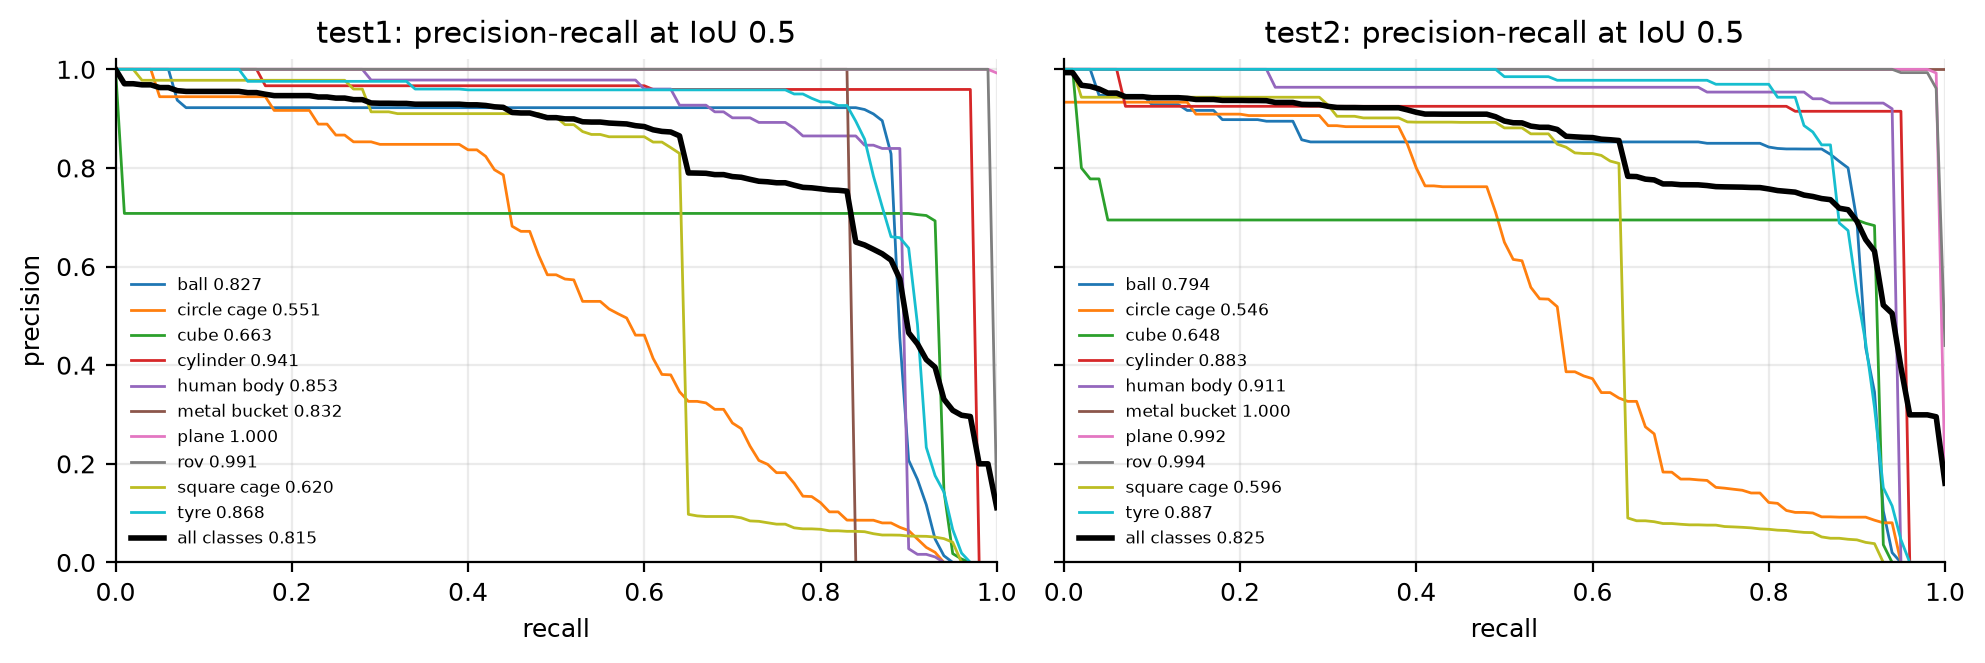
\includegraphics[width=\linewidth]{figures/fig_pr_curves.png}
\caption{Per-class precision--recall curves at IoU 0.5 (pycocotools, all areas). Legend values are AP50.}
\end{figure}

\subsection{Confusion between classes}
\begin{figure}[H]\centering
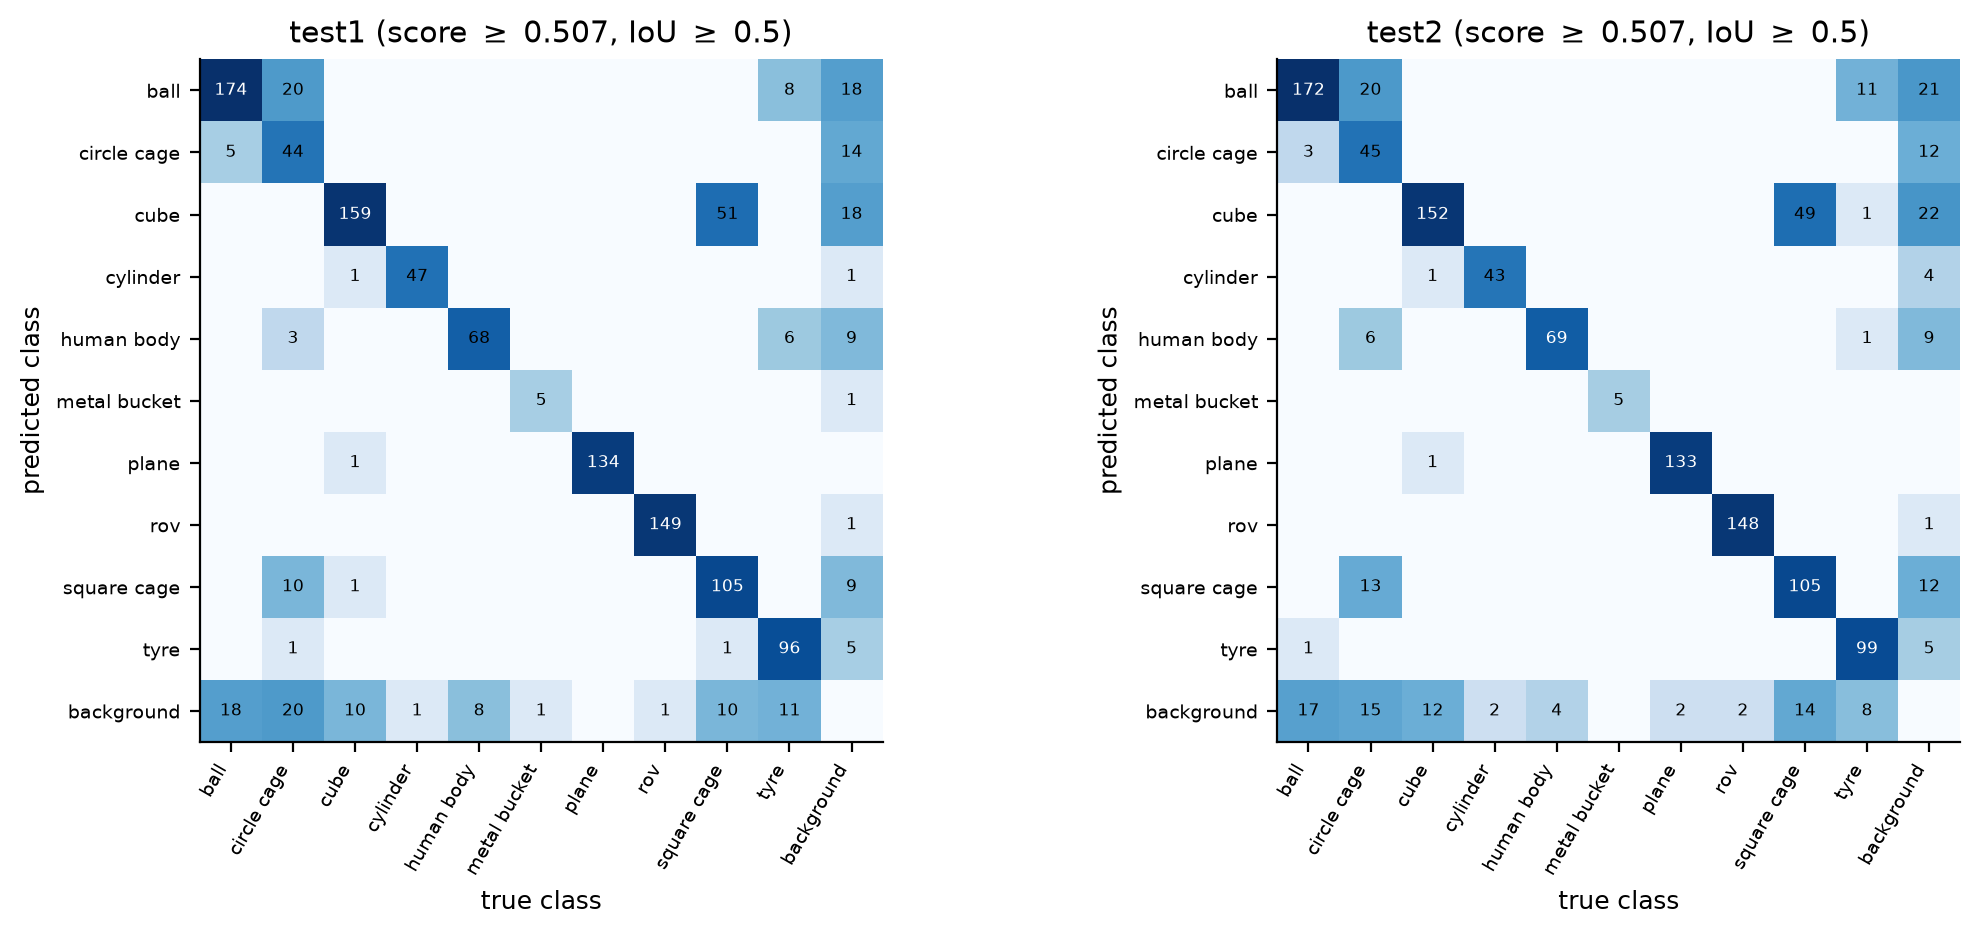
\includegraphics[width=\linewidth]{figures/fig_confusion_test.png}
\caption{Confusion matrices on the test sets. Detections with score $\geq$ 0.507 (the max-F1 confidence chosen on \emph{validation}), class-agnostic one-to-one matching at IoU $\geq$ 0.5. Rows: predicted class; columns: true class; ``background'' = unmatched.}
\end{figure}

\begin{writehere}
Points to cover: the largest error is square cage predicted as cube (51 of 167 square cages in test1, 49 of 168 in test2), which explains cube's flat $\approx$0.7 precision in the PR curve; circle cage is often predicted as ball (20 / 20) or square cage (10 / 13), and missed (20 / 15); missed objects (bottom row) 80 / 76, unmatched detections (right column) 76 / 86.
\end{writehere}

\subsection{Size-stratified results}
\begin{table}[H]\centering
\caption{AP on the UATD-relative size bins (tiny = area $\leq$ 2300\,px$^2$).}
\gentab{tab_size_bins}
\end{table}

\begin{figure}[H]\centering
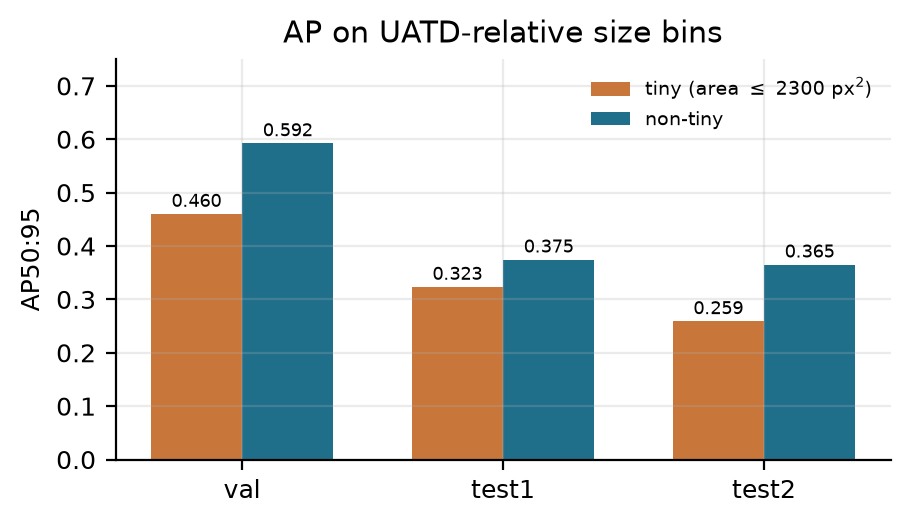
\includegraphics[width=0.6\linewidth]{figures/fig_size_bins.png}
\caption{Tiny versus non-tiny AP50:95.}
\end{figure}

\begin{table}[H]\centering
\caption{Complete COCO-style statistics (pycocotools).}
\gentab{tab_coco_detail}
\end{table}

\begin{writehere}
Points to cover: tiny AP50:95 below non-tiny on every split (test1 0.323 vs 0.375; test2 0.259 vs 0.365); COCO ``small'' bin holds under 1\% of boxes, so AP\textsubscript{S} is noisy; mAP75 far below mAP50, AR at strict IoU low, so box precision is still the main gap; this motivates the tiny-object track (roadmap step 8).
\end{writehere}

\subsection{Qualitative results}
\begin{figure}[H]\centering
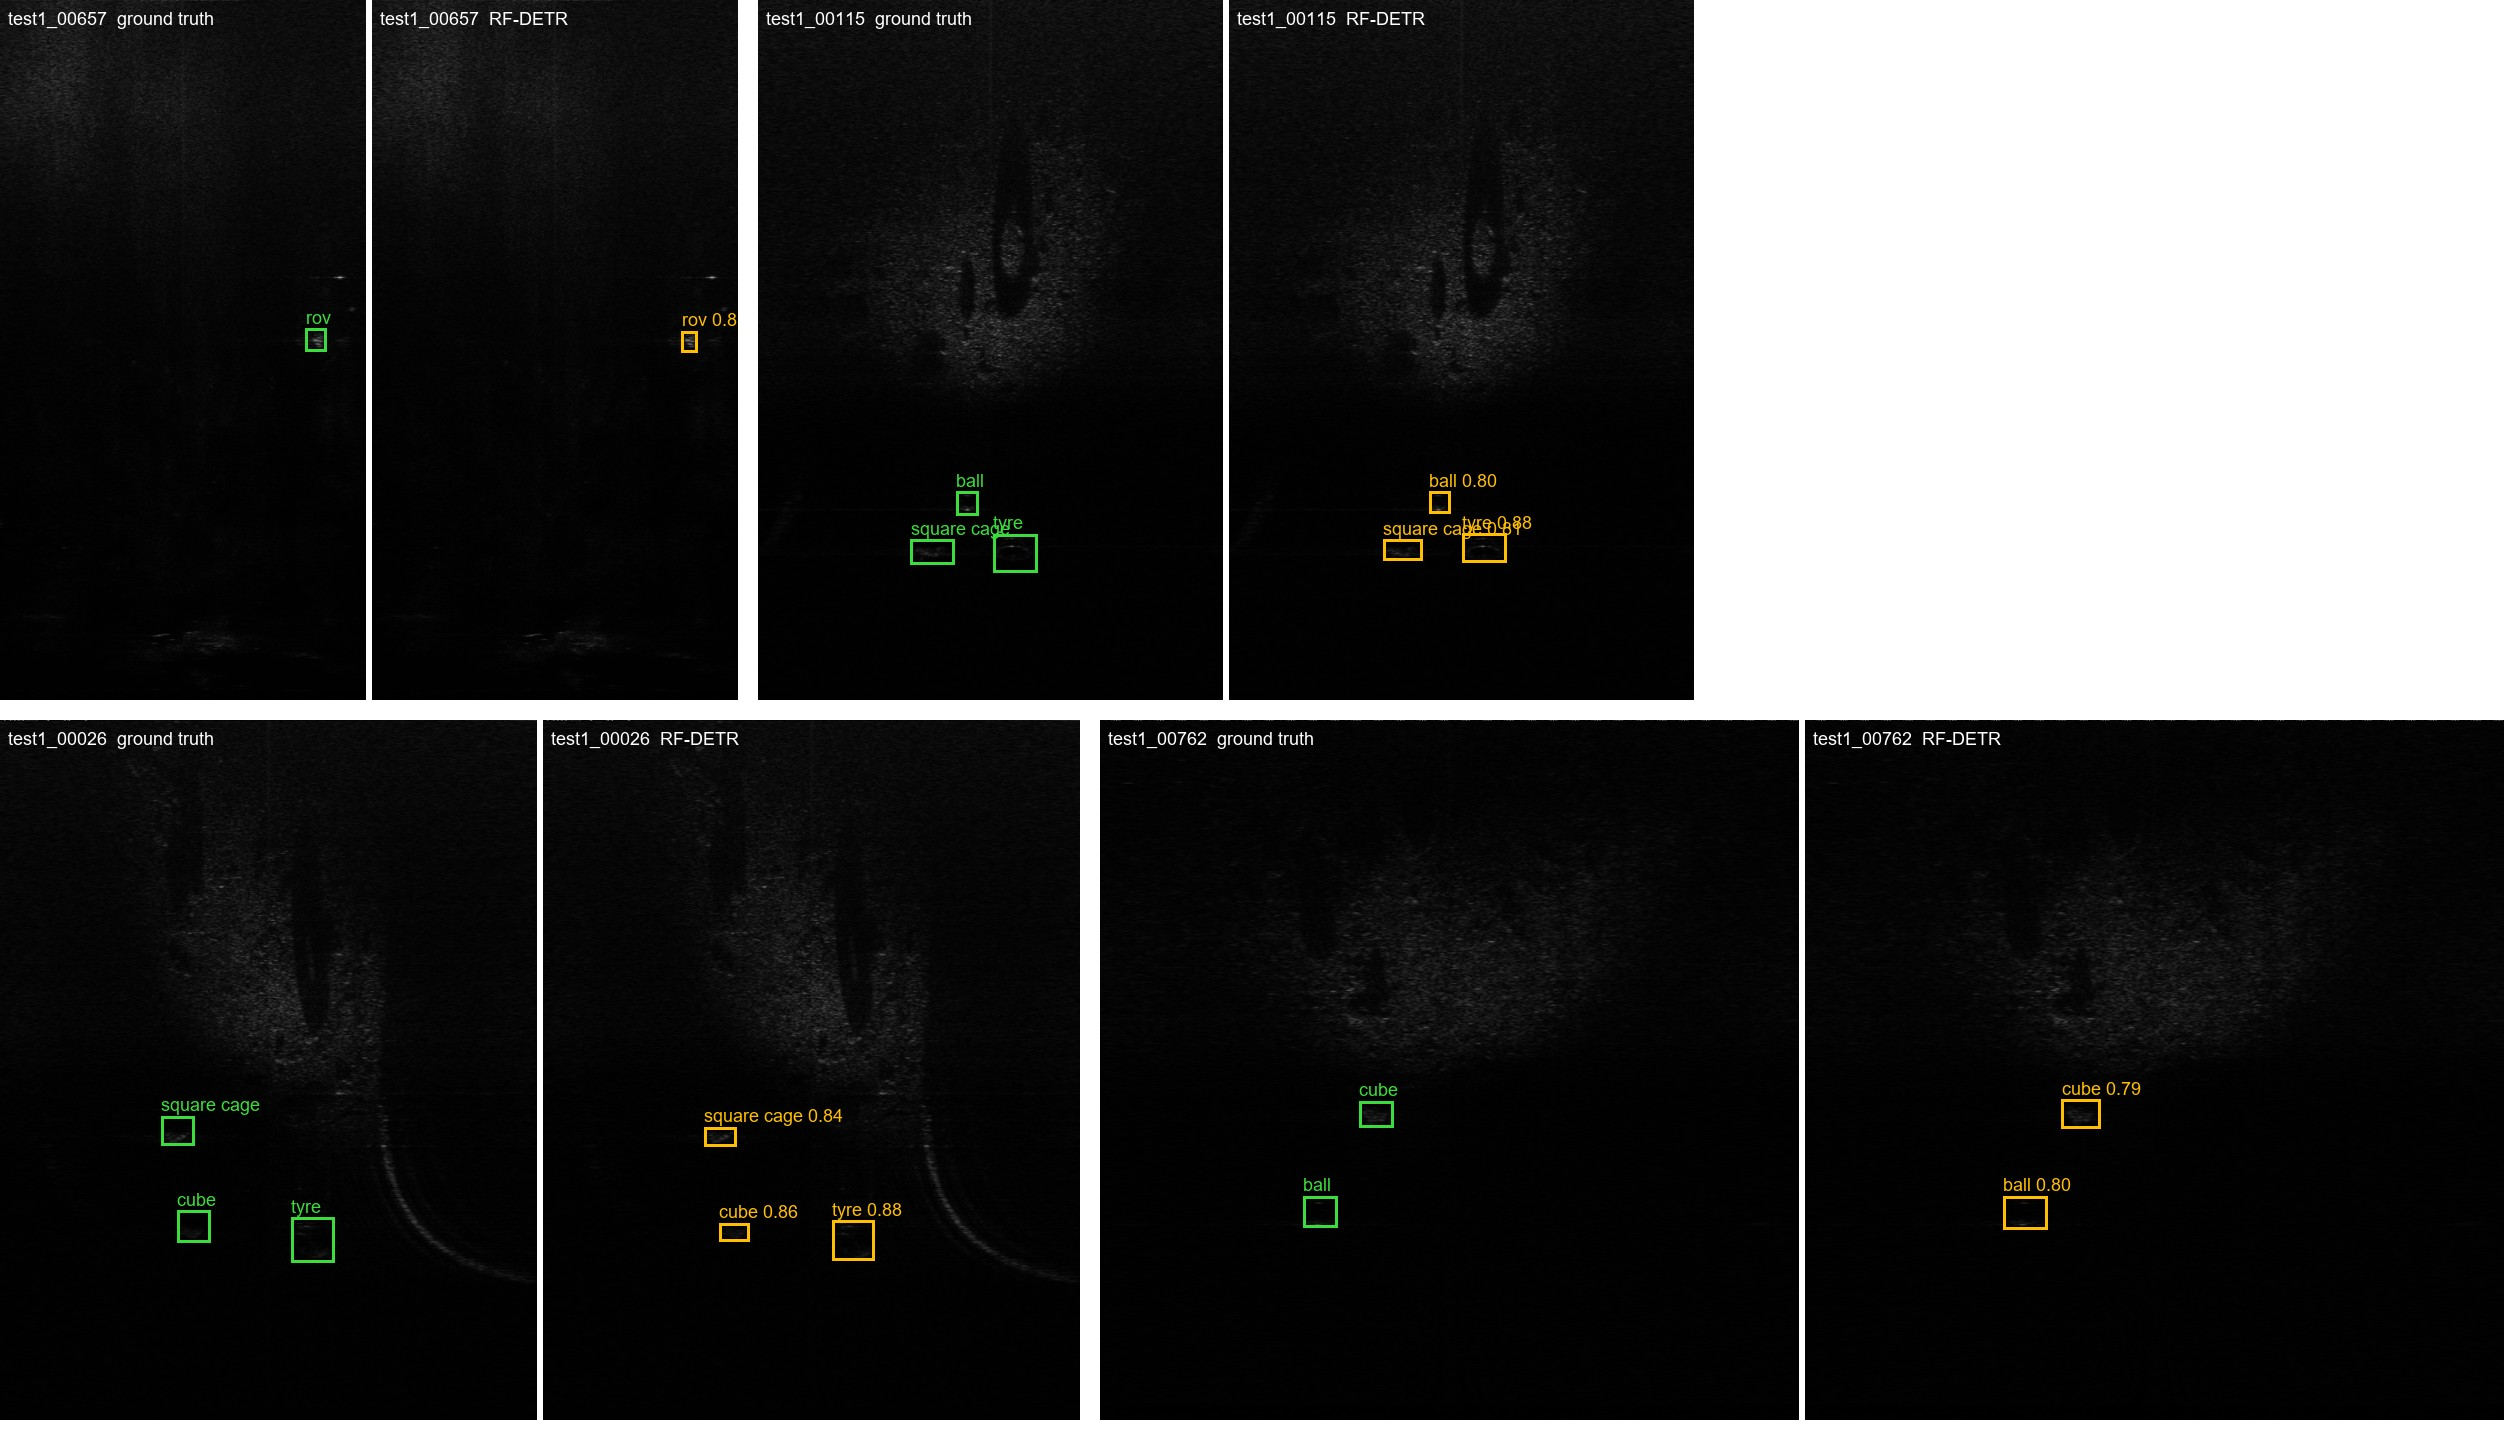
\includegraphics[width=\linewidth]{figures/fig_gallery_test1.jpg}
\caption{Test 1 examples (4 images, seed 42). Green: ground truth. Yellow: RF-DETR detections with score $\geq$ 0.507. Images are shown without contrast change.}
\end{figure}

\begin{figure}[H]\centering
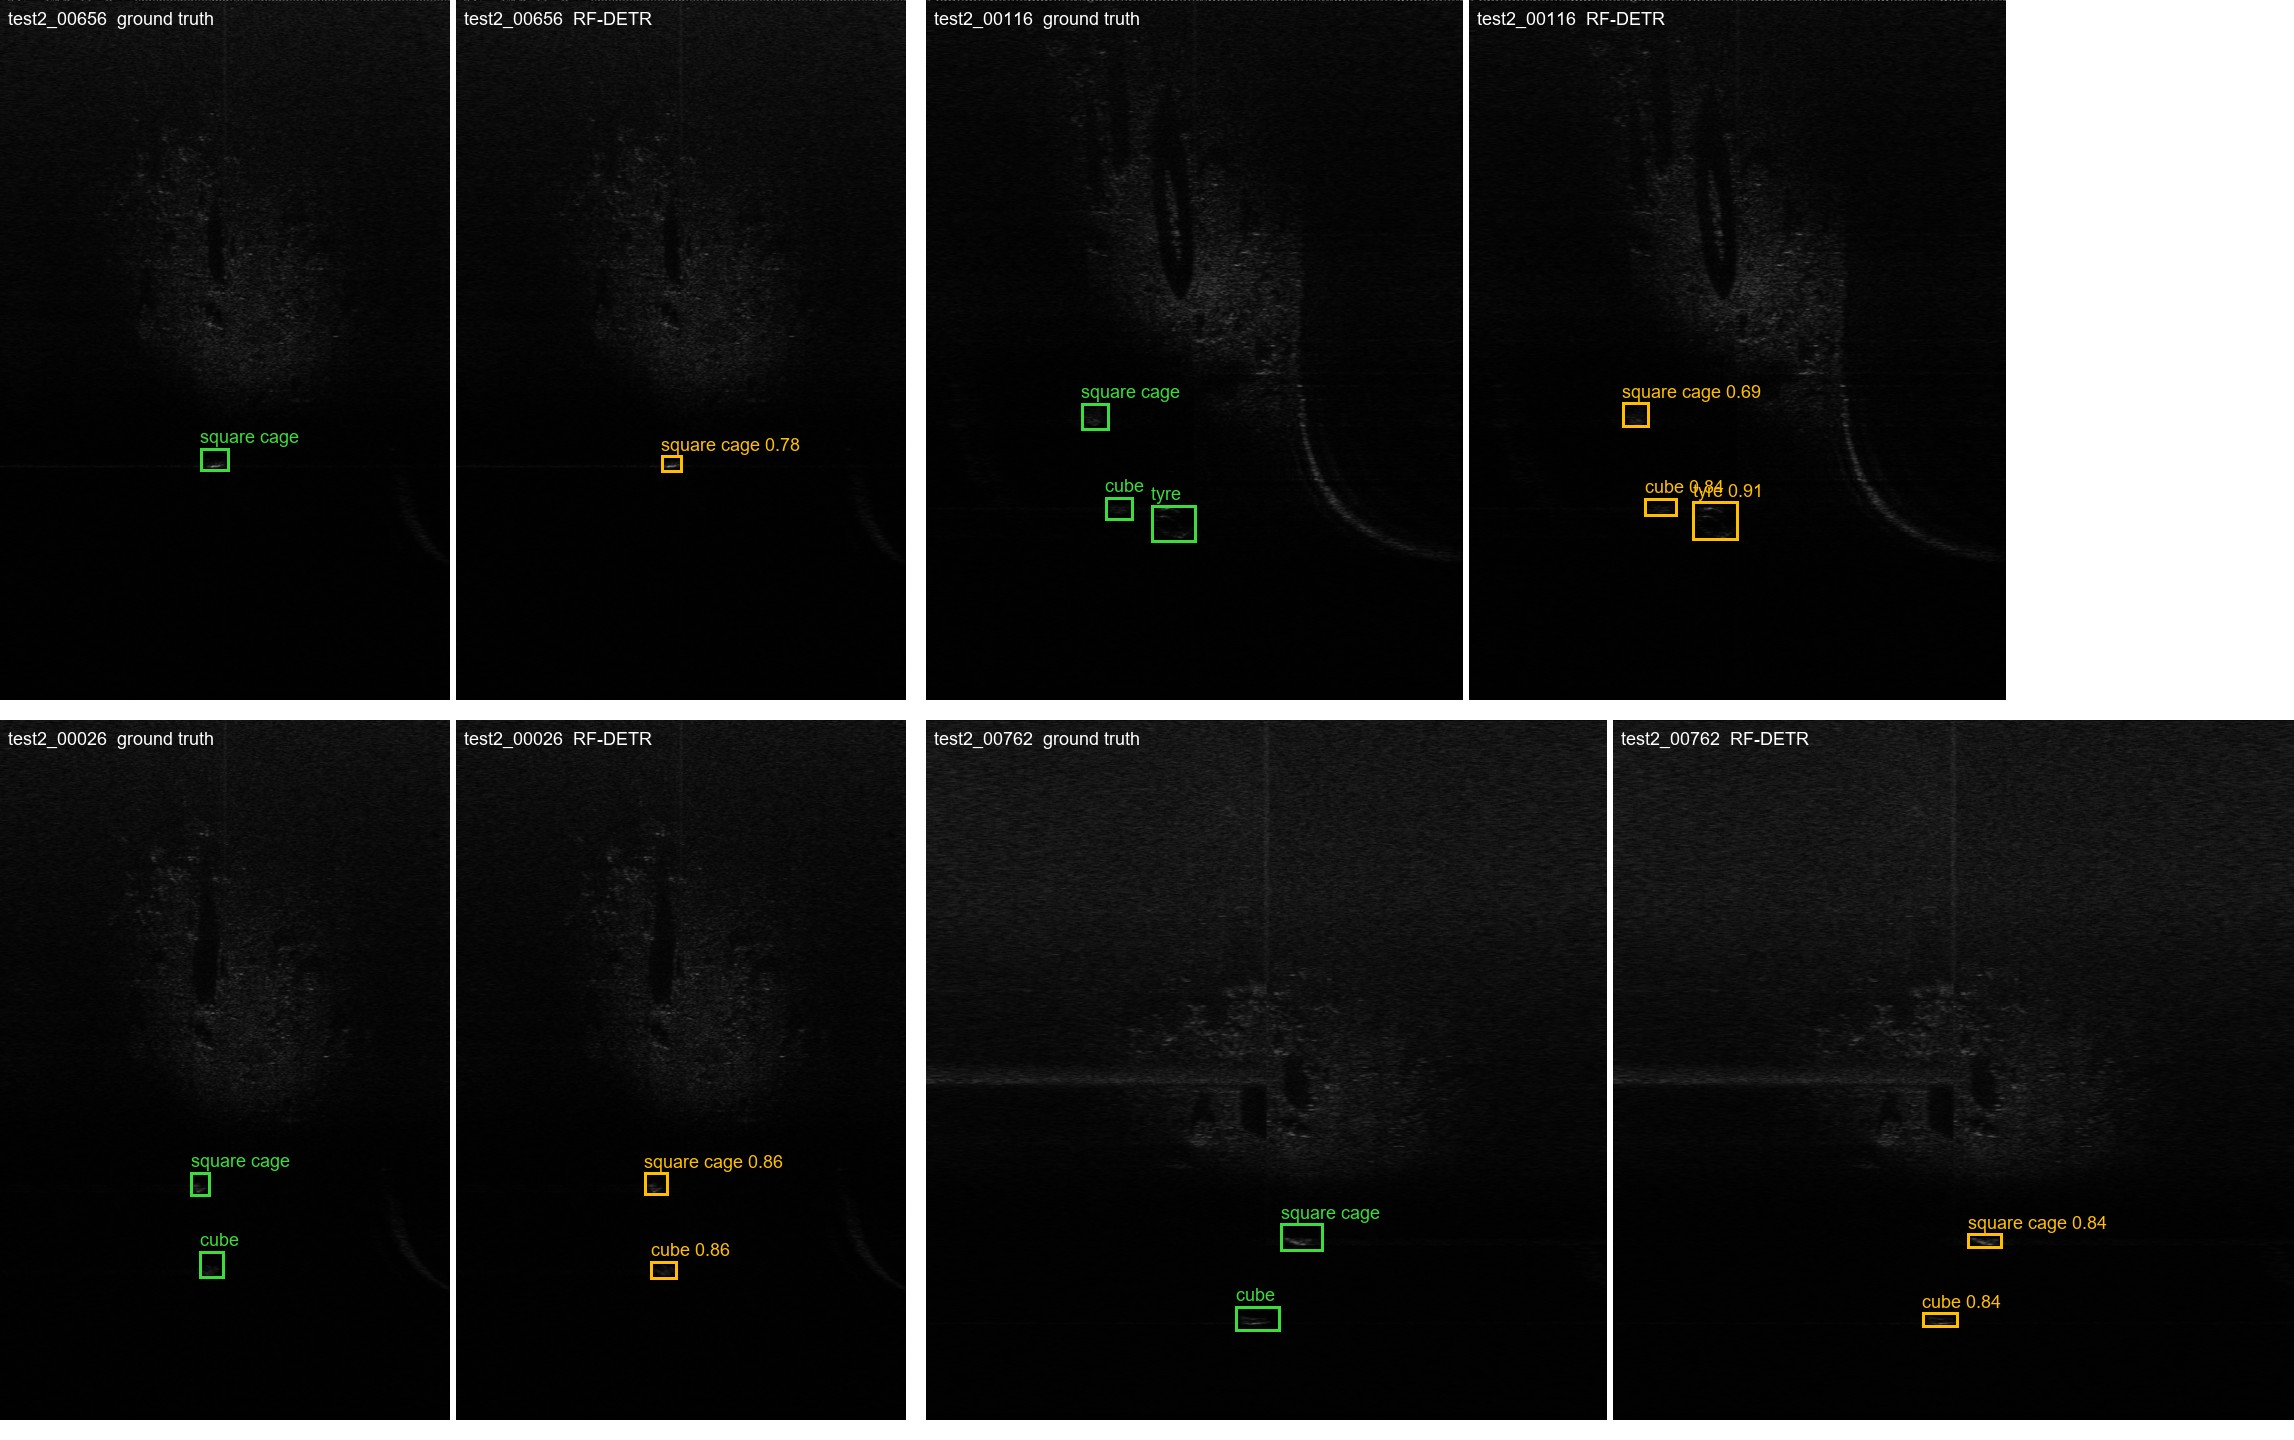
\includegraphics[width=\linewidth]{figures/fig_gallery_test2.jpg}
\caption{Test 2 examples (4 images, seed 42), same convention.}
\end{figure}

% ------------------------------------------------------------------ 6 efficiency
\section{Efficiency}\label{sec:eff}
\begin{table}[H]\centering
\caption{Model complexity and latency. RF-DETR measurements are roadmap step 4 and not done yet.}
\begin{tabular}{lrrrrr}
\toprule
Model & Input & Params (M) & GFLOPs & T4 FP16 (ms) & T4 FP32 (ms)\\
\midrule
YOLO26n$^\dagger$ & 640 & 2.51 & 5.9 & -- & --\\
RF-DETR-S & 512 & pending & pending & pending & pending\\
\bottomrule
\end{tabular}\\[2pt]
{\footnotesize $^\dagger$From the notebook's training model summary; the notebook did not measure batch-1 latency.}
\end{table}

% ------------------------------------------------------------------ 7 discussion
\section{Discussion}
\subsection{What the experiment shows}
\begin{writehere}
Your interpretation of the results above.
\end{writehere}
\subsection{Limitations}
\begin{writehere}
Points to cover: one seed (3 planned); one model size (N and higher resolution pending); efficiency not measured yet; YOLO26n numbers come from Ultralytics' validator, not re-scored with our evaluator (old \texttt{best.pt} not available); random train/val split may share recording sequences, so val is optimistic; test sets are the cleaned 798-image versions.
\end{writehere}
\subsection{Next steps}
\begin{table}[H]\centering
\caption{Planned work (CLAUDE.md roadmap).}
\begin{tabular}{p{4.2cm}p{9.8cm}}
\toprule
Step & Work\\
\midrule
4 Efficiency & params, GFLOPs, batch-1 T4 latency (FP16 / FP32) for every model\\
5 Main pipeline & RF-DETR-N; RF-DETR at higher input resolution\\
6 Baselines & YOLOv12-n/s, FBRT-YOLO, DEIM-D-FINE-S, Dome-DETR on the same split and evaluator\\
7 Error analysis & cage/cube confusion, mAP50--mAP75 gap, tiny-box recall, failure gallery\\
8 Method & one tiny-object idea from an eligible venue on top of RF-DETR, with ablations\\
9 Final runs & 3 seeds for main models, final tables and figures\\
\bottomrule
\end{tabular}
\end{table}

% ------------------------------------------------------------------ appendix
\appendix
\section{Epoch log}\label{app:epochs}
{\small
\setlength{\tabcolsep}{4pt}
\begin{longtable}{rrrrrrrrrr}
\caption{Per-epoch training losses and validation metrics (RF-DETR built-in evaluator).}\\
\toprule
Epoch & Loss & CE & L1 & GIoU & P & R & mAP50 & mAP75 & mAP50:95\\
\midrule
\endfirsthead
\toprule
Epoch & Loss & CE & L1 & GIoU & P & R & mAP50 & mAP75 & mAP50:95\\
\midrule
\endhead
\bottomrule
\endfoot
1 & 6.177 & 0.780 & 0.0278 & 0.297 & 0.911 & 0.907 & 0.930 & 0.389 & 0.464 \\
2 & 5.269 & 0.637 & 0.0239 & 0.268 & 0.943 & 0.920 & 0.936 & 0.448 & 0.493 \\
3 & 5.053 & 0.612 & 0.0229 & 0.259 & 0.957 & 0.937 & 0.947 & 0.489 & 0.519 \\
4 & 4.919 & 0.597 & 0.0223 & 0.252 & 0.967 & 0.943 & 0.961 & 0.505 & 0.524 \\
5 & 4.822 & 0.588 & 0.0217 & 0.247 & 0.949 & 0.951 & 0.955 & 0.511 & 0.529 \\
6 & 4.753 & 0.577 & 0.0208 & 0.244 & 0.973 & 0.949 & 0.961 & 0.540 & 0.538 \\
7 & 4.728 & 0.574 & 0.0211 & 0.242 & 0.958 & 0.954 & 0.961 & 0.552 & 0.545 \\
8 & 4.680 & 0.572 & 0.0204 & 0.239 & 0.965 & 0.946 & 0.962 & 0.565 & 0.545 \\
9 & 4.588 & 0.564 & 0.0202 & 0.233 & 0.962 & 0.957 & 0.960 & 0.578 & 0.552 \\
10 & 4.594 & 0.562 & 0.0201 & 0.233 & 0.965 & 0.952 & 0.962 & 0.558 & 0.549 \\
11 & 4.525 & 0.555 & 0.0196 & 0.230 & 0.963 & 0.959 & 0.967 & 0.581 & 0.557 \\
12 & 4.464 & 0.552 & 0.0192 & 0.227 & 0.970 & 0.963 & 0.969 & 0.582 & 0.559 \\
13 & 4.446 & 0.550 & 0.0193 & 0.226 & 0.967 & 0.966 & 0.969 & 0.594 & 0.562 \\
14 & 4.434 & 0.547 & 0.0189 & 0.227 & 0.973 & 0.960 & 0.965 & 0.597 & 0.563 \\
15 & 4.408 & 0.543 & 0.0192 & 0.224 & 0.977 & 0.969 & 0.969 & 0.581 & 0.561 \\
16 & 4.363 & 0.541 & 0.0187 & 0.221 & 0.977 & 0.966 & 0.969 & 0.606 & 0.568 \\
17 & 4.372 & 0.540 & 0.0190 & 0.222 & 0.979 & 0.960 & 0.969 & 0.602 & 0.567 \\
18 & 4.321 & 0.538 & 0.0186 & 0.218 & 0.972 & 0.966 & 0.966 & 0.588 & 0.563 \\
19 & 4.305 & 0.534 & 0.0185 & 0.218 & 0.967 & 0.968 & 0.967 & 0.599 & 0.564 \\
20 & 4.286 & 0.531 & 0.0185 & 0.217 & 0.956 & 0.971 & 0.971 & 0.595 & 0.569 \\
21 & 4.262 & 0.531 & 0.0180 & 0.215 & 0.968 & 0.969 & 0.969 & 0.587 & 0.567 \\
22 & 4.241 & 0.530 & 0.0182 & 0.214 & 0.965 & 0.968 & 0.970 & 0.587 & 0.570 \\
23 & 4.218 & 0.528 & 0.0179 & 0.212 & 0.970 & 0.969 & 0.967 & 0.613 & 0.576 \\
24 & 4.180 & 0.525 & 0.0176 & 0.210 & 0.974 & 0.974 & 0.969 & 0.612 & 0.574 \\
25 & 4.185 & 0.521 & 0.0178 & 0.210 & 0.977 & 0.965 & 0.969 & 0.622 & 0.579 \\
26 & 4.163 & 0.520 & 0.0177 & 0.209 & 0.974 & 0.970 & 0.968 & 0.631 & 0.580 \\
27 & 4.127 & 0.518 & 0.0175 & 0.207 & 0.968 & 0.972 & 0.969 & 0.620 & 0.579 \\
28 & 4.138 & 0.518 & 0.0176 & 0.208 & 0.967 & 0.974 & 0.968 & 0.627 & 0.579 \\
29 & 4.136 & 0.520 & 0.0175 & 0.208 & 0.968 & 0.971 & 0.969 & 0.620 & 0.577 \\
30 & 4.085 & 0.514 & 0.0171 & 0.205 & 0.970 & 0.972 & 0.968 & 0.605 & 0.575 \\
31 & 4.068 & 0.512 & 0.0170 & 0.204 & 0.977 & 0.967 & 0.969 & 0.617 & 0.575 \\
32 & 4.079 & 0.514 & 0.0172 & 0.205 & 0.972 & 0.973 & 0.967 & 0.611 & 0.576 \\
33 & 4.044 & 0.511 & 0.0169 & 0.203 & 0.974 & 0.965 & 0.966 & 0.631 & 0.582 \\
34 & 4.026 & 0.510 & 0.0166 & 0.201 & 0.970 & 0.967 & 0.964 & 0.612 & 0.575 \\
35 & 4.022 & 0.510 & 0.0168 & 0.201 & 0.975 & 0.957 & 0.967 & 0.627 & 0.579 \\
36 & 4.007 & 0.506 & 0.0166 & 0.200 & 0.973 & 0.966 & 0.970 & 0.626 & 0.579 \\
37 & 3.978 & 0.504 & 0.0163 & 0.199 & 0.975 & 0.966 & 0.968 & 0.612 & 0.579 \\
38 & 3.984 & 0.505 & 0.0164 & 0.198 & 0.971 & 0.970 & 0.967 & 0.623 & 0.580 \\
39 & 3.934 & 0.499 & 0.0161 & 0.197 & 0.975 & 0.969 & 0.969 & 0.633 & 0.583 \\
40 & 3.929 & 0.499 & 0.0163 & 0.196 & 0.976 & 0.968 & 0.970 & 0.643 & 0.585 \\
41 & 3.939 & 0.499 & 0.0163 & 0.196 & 0.970 & 0.974 & 0.970 & 0.636 & 0.582 \\
42 & 3.897 & 0.497 & 0.0160 & 0.193 & 0.972 & 0.969 & 0.971 & 0.626 & 0.582 \\
43 & 3.879 & 0.495 & 0.0159 & 0.193 & 0.975 & 0.968 & 0.970 & 0.622 & 0.578 \\
44 & 3.878 & 0.495 & 0.0159 & 0.192 & 0.972 & 0.973 & 0.968 & 0.615 & 0.579 \\
45 & 3.874 & 0.494 & 0.0158 & 0.192 & 0.971 & 0.970 & 0.967 & 0.635 & 0.583 \\
46 & 3.880 & 0.493 & 0.0160 & 0.192 & 0.980 & 0.969 & 0.973 & 0.638 & 0.587 \\
47 & 3.879 & 0.493 & 0.0159 & 0.192 & 0.975 & 0.967 & 0.967 & 0.628 & 0.584 \\
48 & 3.834 & 0.489 & 0.0156 & 0.190 & 0.971 & 0.969 & 0.970 & 0.629 & 0.586 \\
49 & 3.810 & 0.488 & 0.0155 & 0.187 & 0.976 & 0.972 & 0.974 & 0.632 & 0.587 \\
50 & 3.838 & 0.489 & 0.0157 & 0.189 & 0.974 & 0.972 & 0.973 & 0.646 & 0.588 \\
51 & 3.797 & 0.487 & 0.0153 & 0.188 & 0.975 & 0.970 & 0.969 & 0.627 & 0.584 \\
52 & 3.797 & 0.485 & 0.0155 & 0.187 & 0.971 & 0.970 & 0.971 & 0.630 & 0.582 \\
53 & 3.791 & 0.484 & 0.0153 & 0.187 & 0.968 & 0.971 & 0.968 & 0.640 & 0.584 \\
54 & 3.759 & 0.481 & 0.0154 & 0.184 & 0.972 & 0.973 & 0.969 & 0.638 & 0.588 \\
55 & 3.734 & 0.478 & 0.0150 & 0.184 & 0.977 & 0.972 & 0.970 & 0.639 & 0.584 \\
56 & 3.752 & 0.480 & 0.0153 & 0.185 & 0.975 & 0.971 & 0.966 & 0.626 & 0.585 \\
57 & 3.714 & 0.477 & 0.0149 & 0.183 & 0.975 & 0.968 & 0.967 & 0.634 & 0.580 \\
58 & 3.714 & 0.476 & 0.0150 & 0.183 & 0.971 & 0.977 & 0.970 & 0.629 & 0.585 \\
59 & 3.675 & 0.472 & 0.0148 & 0.181 & 0.968 & 0.980 & 0.970 & 0.613 & 0.583 \\
60 & 3.655 & 0.470 & 0.0145 & 0.180 & 0.975 & 0.973 & 0.969 & 0.606 & 0.579 \\
61 & 3.654 & 0.472 & 0.0145 & 0.178 & 0.975 & 0.973 & 0.971 & 0.629 & 0.579 \\
62 & 3.666 & 0.472 & 0.0149 & 0.179 & 0.974 & 0.966 & 0.967 & 0.615 & 0.580 \\
63 & 3.648 & 0.469 & 0.0146 & 0.179 & 0.979 & 0.971 & 0.971 & 0.613 & 0.577 \\
64 & 3.646 & 0.470 & 0.0145 & 0.178 & 0.975 & 0.969 & 0.966 & 0.606 & 0.579 \\
65 & 3.651 & 0.469 & 0.0147 & 0.178 & 0.981 & 0.964 & 0.968 & 0.625 & 0.580 \\

\end{longtable}
}

\section{Reproducibility}
\begin{table}[H]\centering
\caption{Where everything lives in the repository.}
\begin{tabular}{p{5cm}p{9cm}}
\toprule
Item & Location\\
\midrule
Code & \url{https://github.com/azmineamin/uatd-sonar-detection}\\
Split manifests & \texttt{data/splits/*.txt}\\
Size-bin config (frozen) & \texttt{configs/eval.yaml}\\
Training & \texttt{scripts/train\_rfdetr.py}, \texttt{notebooks/kaggle\_runner.ipynb}\\
Prediction + evaluation & \texttt{scripts/predict\_rfdetr.py}, \texttt{src/uatd/eval\_coco.py}\\
Run metrics & \texttt{results/rfdetr/small\_rdefault\_s0/}\\
This report's assets & \texttt{scripts/make\_report\_assets.py}\\
\bottomrule
\end{tabular}
\end{table}

\end{document}
